\documentclass{cumtthesis}
%****************************
%    中国矿业大学学位论文模板     
%        V2.3.0-Beta
%  支持本、硕、博的学位论文撰写
%****************************
% > 暂不支持外文学院研究生学位论文

% 设置元数据
\cumtsetup{
    %
    %**************************************
    % 注意事项:
    %    1. 不需要的项可以删除(将使用默认值)
    %    2. \cumtsetup{} 内不要留空行
    %**************************************
    %
    %----------------------------------------------------------------
    % 输出格式:默认为 "electronic",可选:
    %    - electronic  [电子版/普通版/存档版](连续无空白页。用于上传中国知网等数据库和上级主管部门论文抽检)
    %    - print       [打印版](增加空白页以便直接双面打印。注意空白页也占用页码。)
    %    - blindreview [盲审版](隐藏敏感信息。用于双盲送审。仅保留封面页和论文主体部分,包含从摘要至作者简介;博士学位论文还应有“创新性评价”内容)
    %    - inspection  [抽检版](用于江苏省学位论文抽检。抽检论文应在存档学位论文的基础上隐去:作者姓名、导师姓名、学校名称、学校代码、培养单位名称、培养单位代码、学位授予单位名称、学位授予单位代码、培养单位地址、邮编、答辩委员会主席、答辩委员会成员等可能辨认出论文来源的字样,有关隐去文字统一用*字符号代替,删除:学校校徽标识、删除致谢部分)
    output = {electronic},
    %----------------------------------------------------------------
    % 封面基金列表:默认为 "false",可选:
    %    - true  显示(矿业、安全等部分学院有此要求)
    %    - false  不显示
    % 注意:此选项仅对研究生有效
    funding-on-cover = {true},
    %----------------------------------------------------------------
    % 论文类型:默认为 "硕士学位论文",可填包括但不限于:
    % 1. 本科生:
    %    - 本科生毕业设计(论文)
    % 2. 学术型研究生:
    %    - 博士学位论文
    %    - 硕士学位论文
    % 3. 专业型研究生:
    %    - 工程硕士专业学位论文
    %    - 公共管理硕士专业学位论文
    %    - 工商管理硕士专业学位论文
    %    - 会计硕士专业学位论文
    %    - 翻译硕士专业学位论文
    %    - 资产评估硕士专业学位论文
    %    - 体育硕士专业学位论文
    %    - 工程管理硕士专业学位论文
    %    - 艺术硕士专业学位论文
    %    - 法律硕士专业学位论文
    %    - 建筑学硕士专业学位论文
    %    - ...
    thesis-type = {硕士学位论文},
    %----------------------------------------------------------------
    % 中文标题:默认为 "论文标题"
    title = {浮选旋流分选机理研究},
    %----------------------------------------------------------------
    % 英文标题:默认为 "Thesis Title"
    title* = {Study on the Cyclonic Separation Mechanism of Flotation},
    %----------------------------------------------------------------
    % 作者姓名:默认为 "姓名"
    author = {陈二},
    %----------------------------------------------------------------
    % 导师姓名:默认为 "姓名"
    supervisor = {张三},
    %----------------------------------------------------------------
    % 导师职称:默认为 "职称"
    supervisor-title = {教授},
    %----------------------------------------------------------------
    % 第二导师姓名[选填]:默认为空
    co-supervisor = {李四},
    %----------------------------------------------------------------
    % 第二导师职称[选填]:默认为空
    co-supervisor-title = {副教授},
    %----------------------------------------------------------------
    % 论文提交年份:默认为 2000
    year = {2025},
    %----------------------------------------------------------------
    % 论文提交月份:默认为 6
    month = {6},
    %----------------------------------------------------------------
    % 培养单位(学院):默认为空
    affiliation = {计算机科学与技术学院},
    %----------------------------------------------------------------
    % 学科专业:默认为空
    major = {计算机科学与技术},
    %----------------------------------------------------------------
    % 学号:默认为空
    student-id = {TS22000000A11},
    %----------------------------------------------------------------
    % 密级:默认为 "公开"
    security-level = {公开},
    %----------------------------------------------------------------
    % 保密期(起讫日期):默认为空(仅涉密论文需要填写)
    confidentiality-period = {},
    %----------------------------------------------------------------
    %********************** 本科生无需填写以下信息 **********************
    %----------------------------------------------------------------
    % 申请学位:默认为空
    degree-applied = {工学硕士},
    %----------------------------------------------------------------
    % 研究方向:默认为空
    field = {人工智能},
    %----------------------------------------------------------------
    % 一级学科(授权点)代码
    first-level-discipline-code = {0812},
    %----------------------------------------------------------------
    % 一级学科(授权点)名称
    first-level-discipline-name = {计算机科学与技术},
    %----------------------------------------------------------------
    % 二级学科(领域)代码
    second-level-discipline-code = {081203},
    %----------------------------------------------------------------
    % 二级学科(领域)名称
    second-level-discipline-name = {计算机应用技术},
    %----------------------------------------------------------------
    % 答辩委员会主席:默认为空
    defense-committee-chair = {王五},
    %----------------------------------------------------------------
    % 答辩委员会成员:默认为空
    defense-committee-members = {赵六、孙七、周八、吴九、郑十},
    %----------------------------------------------------------------
    % 评阅人:默认为空
    reviewer = {校外盲审},
    %----------------------------------------------------------------
    % 中图分类号:默认为空
    clc = {TP123.45},
    %----------------------------------------------------------------
    % UDC 分类号:默认为空
    udc = {001.2},
    %----------------------------------------------------------------
    % 资助信息:默认为空
    % 格式:{<基金名称1>(编号1);<基金名称2>(编号2);<基金名称3>(编号3,编号4)}
    % 注意:使用分号";"分隔。下划线"_"应使用转义字符"\_"。
    funding = {国家重点研发计划项目(0000YFC0000000);国家自然科学基金项目(12345678,87654321);国家自然科学基金联合基金重点项目(12345678);江苏省研究生科研创新计划项目(KYCX24\_1234)}, 
    %----------------------------------------------------------------
    % 学位类别:默认为空
    degree-category = {工学},
    %----------------------------------------------------------------
    % 论文语种:默认为 "中文"
    language = {中文},
    %----------------------------------------------------------------
    % 学制:默认为空
    program-duration = {3年},
    %----------------------------------------------------------------
    % 电子版论文格式[选填]:默认为空,可选:
    %    - 文本
    %    - 图像
    %    - 视频
    %    - 音频
    %    - 多媒体
    %    - 其他
    electronic-thesis-format = {文本},
    %----------------------------------------------------------------
    % 电子版论文出版者[选填]:默认为空
    electronic-thesis-publisher = {},
    %----------------------------------------------------------------
    % 电子版论文出版地[选填]:默认为空
    electronic-thesis-publisher-location = {},
    %----------------------------------------------------------------
    % 授权声明[选填]:默认为空
    permission-statement = {},
    %----------------------------------------------------------------
}

% 参考文献文件
\addbibresource{bibliography.bib} 

% 取消底部对齐(若不需要可删除)
\raggedbottom

\begin{document}
%****************************************************************************
% 注意:
%     1. 研究生:请删除所有标注为[本科生]的内容
%     2. 本科生:请删除所有标注为[研究生]的内容
%     3. 博士生:盲审时使用doctoral.tex
%****************************************************************************
%
%=============================================== 封面和前言部分
\pagestyle{empty}
\MakeCoverPage % 封面
\MakeGraduateCopyrightDeclarationPage % [研究生]使用授权声明
\MakeTitlePage % 扉页
% \MakeUndergraduateDeclarationPages % [本科生]原创性声明、诚信承诺书、使用授权声明

\begin{acknowledgements}

感谢Х Х Х Х Х Х Х Х Х Х Х Х Х Х Х Х Х Х Х Х Х Х Х Х Х Х Х Х Х Х Х Х Х Х Х Х Х Х Х Х Х Х Х Х Х Х Х Х Х Х Х Х Х Х Х Х Х Х Х Х Х Х Х Х Х Х Х Х Х Х Х Х Х Х Х Х Х Х Х Х Х Х Х Х Х Х Х Х Х Х Х Х Х Х Х Х Х Х Х Х Х Х Х Х Х Х Х Х Х Х Х Х Х Х Х Х Х Х Х Х Х Х Х Х Х Х Х Х Х Х Х Х Х Х Х Х Х Х Х Х Х Х Х Х Х Х Х Х Х Х Х 

感谢Х Х Х Х Х Х Х Х Х Х Х Х Х Х Х Х Х Х Х Х Х Х Х Х Х Х Х Х Х Х Х Х Х Х Х Х Х Х Х Х Х Х Х Х Х Х Х Х Х Х Х Х Х Х Х Х Х Х Х Х Х Х Х Х Х Х Х Х Х Х Х Х Х Х Х Х Х Х Х Х Х Х Х Х Х Х Х Х Х Х Х Х Х Х Х Х Х Х Х Х Х Х Х Х Х Х Х Х Х Х Х Х Х Х Х Х Х Х Х Х Х Х Х Х Х Х Х Х Х Х Х Х Х Х Х Х Х Х Х Х Х Х Х Х Х Х Х Х Х Х Х 

\end{acknowledgements} % 致谢
% % [本科生]评阅表格,包括:
%  - 本科毕业设计(论文)任务书
%  - 毕业设计(论文)指导教师评阅书
%  - 毕业设计(论文)评阅教师评阅书
%  - 毕业设计(论文)答辩及综合成绩


% 一些可能用到的宏
% \cumt@title@cn - 论文题目
% \cumt@author - 作者姓名
% \cumt@affiliation - 单位(学院)
% \cumt@major - 专业
% \cumt@student@id - 学号

\makeatletter
%============================================================================ 表1
% 中国矿业大学本科毕业设计(论文)任务书
\chapter*{中国矿业大学本科毕业设计(论文)任务书}
\begin{center}
{%
    \renewcommand\arraystretch{1.667}
    \begin{tabularx}{\textwidth}{|>{\centering\arraybackslash}m{2.0cm}|X|>{\centering\arraybackslash}m{2.0cm}|X|}
        \hline
        \multicolumn{4}{|l|}{设计(论文)题目: \cumt@title@cn} \\
        \hline
        学院 & \cumt@affiliation & 专业年级 & \cumt@major \\
        \hline
        学生姓名 & \cumt@author & 学号 & \cumt@student@id \\
        \hline
        \multicolumn{4}{|l|}{%
            \parbox[t][9cm][l]{\textwidth-2\ccwd}{%
                1、设计(论文)的主要内容

                %******************************
                % 在此处填写<设计(论文)的主要内容>
                %******************************

            }
        } \\
        \hline
        \multicolumn{4}{|l|}{%
            \parbox[t][9cm][l]{\textwidth-2\ccwd}{%
                2、设计(论文)的基本要求

                %******************************
                % 在此处填写<设计(论文)的基本要求>
                %******************************

                \vfill
                \hspace{15\ccwd}指导教师签字:% \includegraphics[width=2.0cm]{path/to/signature.png}
                \vspace{12bp}
            }
        } \\
        \hline
    \end{tabularx}

}
\end{center}
\clearpage
%============================================================================
%============================================================================ 表2
% 中国矿业大学毕业设计(论文)指导教师评阅书
\chapter*{中国矿业大学毕业设计(论文)指导教师评阅书}
\begin{center}
{%
    \renewcommand\arraystretch{1.667}
    \begin{tabularx}{\textwidth}{|>{\centering\arraybackslash}m{3.5cm}|X|>{\centering\arraybackslash}m{2.0cm}|X|}
        \hline
        学生姓名 & \cumt@author & 学号 & \cumt@student@id \\
        \hline
        设计(论文)题目 & \multicolumn{3}{c|}{\cumt@title@cn} \\
        \hline
        \multicolumn{4}{|l|}{%
            \parbox[t][20cm][l]{\textwidth-2\ccwd}{%
                指导教师评语(①基础理论及基本技能的掌握;②独立解决实际问题的能力;③研究内容的理论依据和技术方法;④取得的主要成果及创新点;⑤工作态度及工作量;⑥总体评价及建议成绩;⑦存在问题;⑧是否同意答辩等):

                %*************************
                % 在此处填写<指导教师评语>
                %*************************

                \vfill
                成绩:\hspace{12\ccwd}指导教师签字:% \includegraphics[width=2.0cm]{path/to/signature.png}

                \hspace{20\ccwd} \hspace{2\ccwd}年\hspace{\ccwd}月\hspace{\ccwd}日
                \vspace{12bp}
            }
        } \\
        \hline
    \end{tabularx}

}
\end{center}
\clearpage
%============================================================================
%============================================================================ 表3
% 中国矿业大学毕业设计(论文)评阅教师评阅书
\chapter*{中国矿业大学毕业设计(论文)评阅教师评阅书}
\begin{center}
{%
    \renewcommand\arraystretch{1.667}
    \begin{tabularx}{\textwidth}{|>{\centering\arraybackslash}m{3.5cm}|X|>{\centering\arraybackslash}m{2.0cm}|X|}
        \hline
        学生姓名 & \cumt@author & 学号 & \cumt@student@id \\
        \hline
        设计(论文)题目 & \multicolumn{3}{c|}{\cumt@title@cn} \\
        \hline
        \multicolumn{4}{|l|}{%
            \parbox[t][20cm][l]{\textwidth-2\ccwd}{%
                评阅教师评语(①选题的意义;②基础理论及基本技能的掌握;③综合运用所学知识解决实际问题的能力;④工作量的大小;⑤取得的主要成果及创新点;⑥写作的规范程度;⑦总体评价及建议成绩;⑧存在问题;⑨是否同意答辩等):

                %*************************
                % 在此处填写<评阅教师评语>
                %*************************

                \vfill
                成绩:\hspace{12\ccwd}评阅教师签字:% \includegraphics[width=2.0cm]{path/to/signature.png}

                \hspace{20\ccwd} \hspace{2\ccwd}年\hspace{\ccwd}月\hspace{\ccwd}日
                \vspace{12bp}
            }
        } \\
        \hline
    \end{tabularx}

}
\end{center}
\clearpage
%============================================================================
%============================================================================ 表4
% 中国矿业大学毕业设计(论文)答辩及综合成绩
\chapter*{中国矿业大学毕业设计(论文)答辩及综合成绩}
\begin{center}
{%
    \renewcommand\arraystretch{1.3}
    \begin{tabularx}{\textwidth}{|>{\centering\arraybackslash}m{7cm}|X|X|X|X|X|}
        \hline
        
        \multicolumn{6}{|c|}{答\hspace{2\ccwd}辩\hspace{2\ccwd}情\hspace{2\ccwd}况} \\
        \hline
        \multirow{2}{*}[-3.5ex]{提\hspace{\ccwd}出\hspace{\ccwd}问\hspace{\ccwd}题} & \multicolumn{5}{c|}{回\hspace{\ccwd}答\hspace{\ccwd}问\hspace{\ccwd}题} \\
        \cline{2-6}
        & 正确 & 基本正确 & 有一般性错误 & 有原则性错误 & 没有回答 \\
        \hline
        {} & {$\checkmark$} & {} & {} & {} & {} \\
        \hline
        {} & {$\checkmark$} & {} & {} & {} & {} \\
        \hline
        {} & {$\checkmark$} & {} & {} & {} & {} \\
        \hline
        {} & {$\checkmark$} & {} & {} & {} & {} \\
        \hline
        \multicolumn{6}{|c|}{
            \parbox[t][7cm][l]{\textwidth-2\ccwd}{%
                答辩委员会评语及建议成绩:

                %******************************
                % 在此处填写<答辩委员会评语>
                %******************************
                \vfill
                成绩:\hspace{12\ccwd}答辩委员会主任签字:% \includegraphics[width=2.0cm]{path/to/signature.png}

                \hspace{20\ccwd} \hspace{2\ccwd}年\hspace{\ccwd}月\hspace{\ccwd}日
                \vspace{12bp}
            }
        } \\
        \hline
        \multicolumn{6}{|l|}{成绩评定: ** }\\
        \hline
        \end{tabularx}
        \vskip -1.4pt
        \begin{tabularx}{\textwidth}{|X|X|X|X|X|X|}
        \hline
        \multicolumn{6}{|c|}{成绩评定} \\
        \hline
        成绩组成 & 指导教师 & 评阅教师 & 答辩成绩 & 其他 & 总评 \\
        \hline
        成绩比例 & {} & {} & {} & {} &  \multirow{2}{*}{}\\
        \cline{1-5}
        评分 & {} & {} & {} & {} &  \\
        \hline
        \multicolumn{6}{|c|}{
            \parbox[c][2cm][l]{\textwidth-2\ccwd}{%
                \vfill
                \hspace{15\ccwd}学院领导签字:% \includegraphics[width=2.0cm]{path/to/signature.png}
                \vfill
                \hspace{17\ccwd} \hspace{2\ccwd}年\hspace{\ccwd}月\hspace{\ccwd}日
                \vfill
            }%
        } \\
        \hline
    \end{tabularx}
}
\end{center}
\clearpage
%============================================================================
\makeatother
 % [本科生]任务书、评阅书、答辩成绩表格
% % [博士生]博士论文创新性评价
% 用于双盲评审



% 可能用到的宏和命令
% \cumt@title@cn - 论文题目
% \cumt@clearpage - 根据输出模式清页

% 博士论文创新性评价
% 创新点应与“研究生培养管理信息系统”中填写的一致,每个创新点应控制在 100 字以内。
\makeatletter
\newgeometry{left=2.54cm,right=2.54cm,top=2.54cm,bottom=2.54cm}
\chapter*{\zihao{3}博士论文创新性评价}
\begin{center}
{%  
    \renewcommand\arraystretch{1.667}
    \zihao{-4}
    \begin{tabularx}{\textwidth}{|>{\centering\arraybackslash}m{1.5cm}|X|}
        \hline
        \multicolumn{2}{|l|}{\zihao{4}\bfseries 论文题目: \cumt@title@cn} \\
        \hline
        {\zihao{5}\bfseries 序号} & {\zihao{4}\bfseries 作者自述论文中主要的创新点} \\
        \hline
        \parbox[c][4.75cm][c]{\linewidth}{\centering 1\par} & \parbox[c][4.25cm][c]{\linewidth}{%
                %*******************
                % 在此处填写<创新点1>
                旋流-静态微泡浮选是一种具有我国自主知识产权的新型柱式分选方法与设备。特有的旋流场结构以及在煤炭分选方面的成功应用,为浮选柱技术在我国矿物分选方面的拓展奠定了良好的基础。
                %*******************
            } \\ 
        \hline
        \parbox[c][4.75cm][c]{\linewidth}{\centering 2\par} & \parbox[c][4.25cm][c]{\linewidth}{%
                %*******************
                % 在此处填写<创新点2>
                %*******************
            } \\
        \hline
        \parbox[c][4.75cm][c]{\linewidth}{\centering 3\par} & \parbox[c][4.25cm][c]{\linewidth}{%
                %*******************
                % 在此处填写<创新点3>
                %*******************
            } \\
        \hline
        \parbox[c][4.75cm][c]{\linewidth}{\centering 4\par} & \parbox[c][4.25cm][c]{\linewidth}{%
                %*******************
                % 在此处填写<创新点4>
                %*******************
            } \\
        \hline
    \end{tabularx}

}
\end{center}
\cumt@clearpage
\restoregeometry
 % [博士生-盲审]博士论文创新性评价表格
%===============================================
%
%=============================================== 罗马页码部分
\pagestyle{frontmatter}
%% 中文摘要
\begin{cnabstract}
旋流-静态微泡浮选是一种具有我国自主知识产权的新型柱式分选方法与设备。特有的旋流场结构以及在煤炭分选方面的成功应用,为浮选柱技术在我国矿物分选方面的拓展奠定了良好的基础。

X X X X X X X X X X X X X X X X X X X X X X X X X X X X X X X X X X X X X X X X X X X X X X X X X X X X X X X X X X X X X X X X X X X X X X X X X X X X X X X X X X X X X X X X X X X X X X X X X X X X X X X X X X X X X X X X X X X X X X X X X X X X X X X X X X X X X X X X X X X X X X X X X X X X X X X 

\cnkeywords{浮选;旋流;分选机理;浮选动力学;矿物分选}
\end{cnabstract}


%% 英文摘要
\begin{enabstract}
Young college students are the hope of our country and nation. The historical experience shows that the value education problem for the younger generation cannot be neglected at any time and in any environment. Only through the strengthening of core socialist value belief of the youth, especially young college students, the great mission of achievement of great rejuvenation of the Chinese nation will have reliable backup forces.

Cyclonic static micro-bubble flotation is a new column separation method and device with China self-owned intellectual property.  The successful application of this equipment in coal preparation along with its special cyclonic field structure has laid a solid base for the further application of column flotation in mineral processing.

\enkeywords{flotation; cyclonic separation; separation mechanism; flotation kinetics; mineral separation}
\end{enabstract}
\MakeCnContents % 中文目录
\MakeEnContents % 英文目录
\MakeListOfFigures % 图清单
\MakeListOfTables % 表清单
% 变量注释表
\begin{denotation}
    
\Variable{$V_{1}$}{反应器入口速度(m/s)}
\Variable{$t$}{时间,时间间隔,持续时间(s)}
\Variable{$F$}{力(N)}
\Variable{$\gamma$}{表面张力(N/m)}

\end{denotation} % 变量注释表
%===============================================
%
%=============================================== 正文部分
\pagestyle{mainmatter}
\bichapter{绪论}{Introduction}
\bisection{概述}{Overview}
……

……

……

\subsection{研究目标}
描述旋流-静态微泡浮选柱的旋流场结构,分析旋流场特征及其影响\cite{acharya2020acid};借助流体力学软件对柱体的内部流场进行模拟并分析其流场速度分布规律,研究循环矿浆量及给矿量等因素对流场的影响\cite{betz2015coal,li2021characteristics};通过对旋流场内的颗粒受力分析,建立基于旋流的颗粒动力学方程\cite{mohutsiwa2015parametric,xie2012research,中国社会科学院台湾史研究中心2012台湾光复六十五周年暨抗战史实学术研讨会论文集};系统揭示旋流分选作用,并进行相关动力学分析\cite{younger2004environmental,关立哲2014科技期刊编辑审读中要注重比较思维的科学运用}…

……

……

\vspace*{3cm} %空白


\subsection{研究方法}

流场模拟及分选机理研究\cite{谢和平20192025年中国能源消费及煤炭需求预测}。

\begin{table}[H]
    \renewcommand\arraystretch{1.259}
    \centering
    \bicaption{表名\cite{younger2004environmental}}{Table title}
    \label{table: table_1}  
    \begin{tabularx}{0.8\textwidth}{m{3cm}XXXX}
        \toprule[1.5pt]
        标题(mm)       & 占比(\%)   & 标题(\%) & 占比(\%)   & 标题(\%) \\
        \midrule[0.75pt]
        >0.5        & 3.80   & 7.38 & 3.80   & 7.38 \\
        0.5~0.25    & 4.55   & 4.56 & 8.35   & 5.84 \\
        0.25~0.125  & 3.32   & 5.47 & 11.67  & 5.74 \\
        0.125~0.074 & 4.74   & 3.63 & 16.41  & 5.13 \\
        0.074~0.045 & 10.72  & 3.11 & 27.13  & 4.33 \\
        <0.045      & 72.87  & 4.64 & 100.00 & 4.56 \\
        合计          & 100.00 & 4.56 & -      & -   \\
        \bottomrule[1.5pt]
    \end{tabularx}
\end{table}

……

……

\begin{figure}
    \centering
    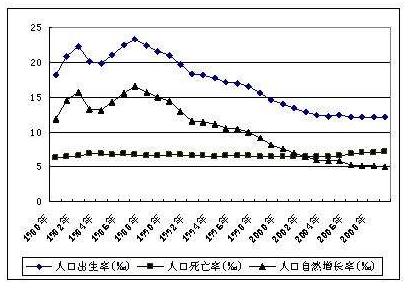
\includegraphics[width=10cm]{Figures/example_fig_1.png}
    \label{fig: fig_1}
    \bicaption{图名}{Figure title}
\end{figure}

描述旋流-静态微泡浮选柱的旋流场结构\footnote{当论文中的字、词或短语等,需要进一步加以说明,而又没有具有的文献来源时,用注释。},分析旋流场特征及其影响;借助流体力学软件对柱体的内部流场进行模拟并分析其流场速度分布规律,研究循环矿浆量及给矿量等因素对流场的影响;\footnote{当论文中的字、词或短语等,需要进一步加以说明,而又没有具有的文献来源时,用注释。}通过对旋流场内的颗粒受力分析,建立基于旋流的颗粒动力学方程;系统揭示旋流分选作用,并进行相关动力学分析…

……

……

……

……

……

……

……

……

……

……

……

……

……
 % 简介
\bichapter{模板使用说明}{Template Usage Guide}
\bisection{简介}{Overview}

该 \LaTeX 模板按照\href{https://gs.cumt.edu.cn/info/1049/3149.htm}{《中国矿业大学研究生学位论文撰写规定及模板(2021年版)》}的要求编写(以下简称《撰写规定》)。目前支持硕士、博士毕业论文撰写(暂不支持外文学院硕士毕业论文)。

\bisection{文档类}{Document Class and Options}
在文档开始时,需指定文档类为:
\begin{center}
    \texttt{\textbackslash documentclass\{cumt-graduate-thesis\}}
\end{center}


\bisection{元数据配置}{Metadata Configuration}
\label{section: metadata configuration}
在文档的导言区,使用 \texttt{\textbackslash cumtsetup\{\}} 配置论文的元数据。以下是一些关键配置项:

\begin{itemize}
    \item \texttt{output}:设置输出格式,可选 \texttt{electronic}(电子版)或 \texttt{print}(打印版)。
    \item \texttt{funding-on-cover}:是否在封面显示基金信息,可选 \texttt{true} 或 \texttt{false}。
    \item \texttt{title} 和 \texttt{title*}:分别设置中文标题和英文标题。
    \item \texttt{author}:设置作者姓名。
    \item \texttt{thesis-name}:设置论文类型,如“硕士学位论文”或“博士学位论文”。
    \item \texttt{supervisor} 和 \texttt{supervisor-title}:设置导师姓名和职称。
    \item \texttt{co-supervisor} 和 \texttt{co-supervisor-title}:设置第二导师姓名和职称(选填)。
    \item \texttt{year} 和 \texttt{month}:设置论文提交的年月。
    \item \texttt{degree-applied}:设置申请学位的名称。
    \item \texttt{affiliation}:设置培养单位。
    \item \texttt{major}:设置学科专业。
    \item \texttt{field}:设置研究方向。
    \item \texttt{defense-committee-chair}:设置答辩委员会主席。
    \item \texttt{reviewer}:设置评阅人。
    \item \texttt{security-level}:设置密级,默认为“公开”。
    \item \texttt{clc}:设置中图分类号。
    \item \texttt{udc}:设置 UDC 分类号(选填)。
    \item \texttt{funding}:设置资助信息,格式为 \texttt{\{<基金名称1>(编号1);<基金名称2>(编号2);...\}}。
    \item \texttt{degree-category}:设置学位类别。
    \item \texttt{degree-level}:设置学位级别。
    \item \texttt{language}:设置论文语种,默认为“中文”。
    \item \texttt{student-id}:设置学号。
    \item \texttt{program-duration}:设置学制。
    \item \texttt{defense-committee-members}:设置答辩委员会成员(选填)。
    \item \texttt{electronic-thesis-format}:设置电子版论文格式(选填)。
    \item \texttt{electronic-thesis-publisher}:设置电子版论文出版者(选填)。
    \item \texttt{electronic-thesis-publisher-location}:设置电子版论文出版地(选填)。
    \item \texttt{permission-statement}:设置授权声明(选填)。
\end{itemize}

\bisection{多级标题}{Titles}
使用以下命令输入各级标题:
\begin{itemize}[itemsep=2pt,topsep=5pt]
    \item \verb|\bichapter{}{}|:中文、英文一级标题(章)。
    \item \verb|\bisection{}{}|:中文、英文二级标题(节)。
    \item \verb|\subsection{}|:三级标题(小节)。
    \item \verb|\subsubsection{}|:四级标题(次小节)\footnote{《撰写规定》中未对四、五、六级标题作具体要求}。
    \item \verb|\paragraph{}|:五级标题(段落)。默认为内嵌(Run-in)标题,可使用\verb|\paragraph*{}|实现陈列(Display)标题。
    \item \verb|\subparagraph{}|:六级标题(小段)。默认为内嵌(Run-in)标题,可使用\verb|\subparagraph*{}|实现陈列(Display)标题。
\end{itemize}

\bisection{内容和章节}{Contents and Chapters}

\subsection{封面与扉页}
\begin{itemize}[itemsep=2pt,topsep=5pt]
    \item \verb|\MakeCoverPage|:生成封面页。
    \item \verb|\MakeTitlePage|:生成扉页。
\end{itemize}

封面与扉页信息来自于元数据(见\ref{section: metadata configuration}),因此请确保所有必要字段都已正确填写。

\subsection{学位论文使用授权声明}
通过\verb|\MakeCopyrightPage|命令生成。

\subsection{致谢}
致谢部分放置在\texttt{acknowledgements.tex},使用\texttt{acknowledgements}环境。

\subsection{摘要与关键词}
\begin{itemize}[itemsep=2pt,topsep=5pt]
    \item \verb|\begin{cnabstract}...\end{cnabstract}|:定义中文摘要。
    \item \verb|\begin{enabstract}...\end{enabstract}|:定义英文摘要。
    \item \verb|\cnkeywords{}|:定义中文关键词(需要被包裹于\texttt{cnabstract}环境内)。
    \item \verb|\enkeywords{}|:定义英文关键词(需要被包裹于\texttt{enabstract}环境内)。
    \item \verb|\MakeCnAbstract|:生成中文摘要页面。
    \item \verb|\MakeEnAbstract|:生成英文摘要页面。
\end{itemize}

\subsection{目录}
\begin{itemize}[itemsep=2pt,topsep=5pt]
    \item \verb|\MakeCnContents|:生成中文目录。
    \item \verb|\MakeEnContents|:生成英文目录。
\end{itemize}

\subsection{图表清单}
\begin{itemize}[itemsep=2pt,topsep=5pt]
    \item \verb|\MakeListOfFigures|:生成图清单。
    \item \verb|\MakeListOfTables|:生成表清单。
\end{itemize}

\subsection{变量注释表}
变量注释表放置在\texttt{denotation.tex},使用\texttt{denotation}环境,并使用\verb|\Variable{}{}|命令依次添加符号和解释。

\subsection{正文内容}
正文部分每个章节应保存为单独的.tex文件,并通过\verb|\input{}|命令引入主文档中。

\subsection{脚注}
使用\verb|\footnote{}|命令插入脚注\footnote{脚注示例}。

\subsection{参考文献}
参考文献列表由\verb|\MakeReferencePage|命令生成,并按照GB/T-7714标准进行引用格式化。使用\verb|\addbibresource{}|在导言区指定bib文件。

\subsection{附录}
附录用于包含补充材料(非必须)。该部分放置在\texttt{appendix.tex},需使用\texttt{appendix}环境。

\subsection{简历}
简历部分放置在\texttt{resume.tex},需使用\texttt{resume}环境\footnote{使用\texttt{\textbackslash resumesection{}}命令添加小节标题。}。

\subsection{原创性声明}
原创性声明页可通过\verb|\MakeDeclarationPage|命令生成。

\subsection{学位论文数据集}
学位论文数据集页面由\verb|\MakeDataCollectionPage|命令生成,其中包含了论文的各项元数据信息,如密级、分类号、资助项目等。

\bisection{浮动体}{Floats}
\subsection{图}
模板使用 \textsf{subcaption} 宏包实现子图。具体用法参考\url{https://mirrors.ibiblio.org/CTAN/macros/latex/contrib/caption/subcaption.pdf}

\subsection{表}
......

\subsection{算法}
模板中使用 \texttt{algorithm2e} 宏包实现算法环境。具体用法参考官方文档。

\begin{algorithm}
  \SetAlgoLined
  \KwData{this text}
  \KwResult{some text }
  $x:=x_{0}$\;
  \While{$x<100$}{
    $x:=y^2$\;
    \eIf{$x>a$}{
      $y:=y-1$\;
      $c:=10290$\;
    }{
      $y:=y/2$\;
    }
  }
  \caption{**算法}
  \label{algo:algorithm1}
\end{algorithm}

\nocite{*} % 创新点1
\input{Chapters/work-2} % 创新点2
\input{Chapters/work-3} % 创新点3
% \input{Chapters/work-4} % 创新点4
% ...
\bichapter{结论}{Conclusion}
本文从自然因素、外部环境和内部结构等方面,详细分析了影响我国煤炭供给和需求的因素,探索煤炭供需与其影响因素的规律,构建了我国煤炭供需预测预警指标体系,对我国煤炭供需进行预测预警。

我国的煤炭供给受许多因素度影响,而且随着时间的推移,出现新的特点。

……

……

……

……

……

……

……

……

……

……

……

……

……

……

……

目前,我国的铁路运输压力又所缓解,但铁路运输还是制约着我国的煤炭供给。我国煤炭资源区域分异现象与经济区域分异性相悖,由此造成了“西煤东调”和“北煤南运”的运输格局,这种能源中心与经济中心的差异性,形成了大量的煤炭运输需求以及非常集中的煤炭流量,但因资金的缺口及体制的原因,铁路运输现在将来一段时期都制约着我国的煤炭供给。

目前,我国的铁路运输压力又所缓解,但铁路运输还是制约着我国的煤炭供给。我国煤炭资源区域分异现象与经济区域分异性相悖,由此造成了“西煤东调”和“北煤南运”的运输格局,这种能源中心与经济中心的差异性,形成了大量的煤炭运输需求以及非常集中的煤炭流量,但因资金的缺口及体制的原因,铁路运输现在将来一段时期都制约着我国的煤炭供给。

目前,我国的铁路运输压力又所缓解,但铁路运输还是制约着我国的煤炭供给。我国煤炭资源区域分异现象与经济区域分异性相悖,由此造成了“西煤东调”和“北煤南运”的运输格局,这种能源中心与经济中心的差异性,形成了大量的煤炭运输需求以及非常集中的煤炭流量,但因资金的缺口及体制的原因,铁路运输现在将来一段时期都制约着我国的煤炭供给。


……

……

……

……

……

……

……

……

……

……

……

……

……

……

……

……

……

……

……

……

……

……

……

……

……

……

……

……

……

……

……

……

……

……

……

……

……

……

……

……

……

……

……

……

……
 % 总结展望
%===============================================
%
%=============================================== 附加部分
\pagestyle{backmatter}
\MakeReferencePage % 参考文献
% % [本科生]翻译部分

\bichapter*{翻译部分}{Translation}

{\noindent\heiti\zihao{3}\bfseries 英文原文\par}  

%***********************
% 在此处写<英文原文>
%***********************
\vspace*{10cm}
% \clearpage

{\noindent\heiti\zihao{3}\bfseries 中文译文\par}  

%***********************
% 在此处写<中文译文>
%***********************
\vspace*{10cm}
\clearpage

 % [本科生]翻译部分
%% 附录1
\begin{appendix}

\begin{lstlisting}[language = C]
Imports System.Math
Imports System.Drawing
Public Class Form1

    Private Sub Form1_Load(ByVal sender As System.Object, ByVal e As System.EventArgs) Handles MyBase.Load
        With Grid1
            .Cols = 9
            .Rows = 40
\end{lstlisting}

\end{appendix}



%% 附录2
\begin{appendix}

Some Figures...

\end{appendix} % 附录
% [研究生]个人简历
\begin{resume}

\resumesection{基本情况}
姓名 :\@author \quad 性别:男 \quad 民族:汉 \quad 出生年月:1976-07-23 \quad 籍贯:江苏省东台市 \par
\begin{itemize}
    \setlength{\itemindent}{5.4em}
    \item[] 1995-09—1999-07  中国矿业大学化工学院学士;
    \item[] 1999-09—2002-06  中国矿业大学化工学院攻读硕士学位
\end{itemize}

\resumesection{学术论文}
\begin{enumerate}
    \setlength{\itemindent}{-1.5em}
    \item **. 煤泥脱硫技术现状[J]. 煤泥脱硫技术,2004(1):53-55.
    \item **. 黄铁矿显微赋存特征对浮选脱硫的影响[J]. 煤技术,2005 (5):6-7.
\end{enumerate}

\resumesection{获奖情况}
\begin{enumerate}
    \setlength{\itemindent}{-1.5em}
    \item **. 旋流-静态微泡柱分离方法研究与旋流-静态微泡浮选床研制. 中国机械工业科技进步奖二等奖;
    \item .......
\end{enumerate}

\resumesection{研究项目}
\begin{enumerate}
    \setlength{\itemindent}{-1.5em}
    \item 废弃煤泥的洁净加工与利用.国家重点技术创新项目, 编号:国经贸技术(1999)598号,参加人员;
    \item .......
\end{enumerate}

\end{resume} % [研究生]简历
\MakeGraduateOriginalityDeclarationPage % [研究生]原创性声明
\MakeDataCollectionPage % [研究生]学位论文数据集
%===============================================

\end{document}